%!TEX TS-program = xelatex
%!TEX encoding = UTF-8 Unicode

\documentclass[11pt,tikz,border=1]{standalone}
\usepackage{graphicx}
\usepackage[default,mdseries=Light,bfseries=Medium,path=fonts]{cjkfonts}
\usetikzlibrary{calc,positioning,arrows.meta}

\begin{document}
  \begin{tikzpicture}[
    neuron/.style={circle,draw,thick,inner sep=0pt,minimum size=20mm}
    ]
    
    \node(input1) [neuron] {
    	\scalebox{1.8}{
\includegraphics{pixmap/input_pixels_1}}
    };
    \node(input2) [neuron,right=of input1] {
    	\scalebox{1.8}{
\includegraphics{pixmap/input_pixels_2}}
    };
    \node(input3) [neuron,right=of input2] {
    	\scalebox{1.8}{
\includegraphics{pixmap/input_pixels_3}}
    };
    
    \node(layer1st1) [neuron,above=1.5 of input1] {
    	\scalebox{1.8}{
\includegraphics{pixmap/edges_1}}
    };
    \node(layer1st2) [neuron,above=1.5 of input2] {
    	\scalebox{1.8}{
\includegraphics{pixmap/edges_2}}
    };
    \node(layer1st3) [neuron,above=1.5 of input3] {
    	\scalebox{1.8}{
\includegraphics{pixmap/edges_3}}
    };

    \node(layer2nd1) [neuron,above=1.5 of layer1st1] {
    	\scalebox{1.8}{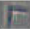
\includegraphics{pixmap/corners_and_contours_1}}
    };
    \node(layer2nd2) [neuron,above=1.5 of layer1st2] {
    	\scalebox{1.8}{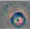
\includegraphics{pixmap/corners_and_contours_2}}
    };
    \node(layer2nd3) [neuron,above=1.5 of layer1st3] {
    	\scalebox{1.8}{
\includegraphics{pixmap/corners_and_contours_3}}
    };

    \node(layer3rd1) [neuron,above=1.5 of layer2nd1] {
    	\scalebox{1.8}{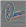
\includegraphics{pixmap/object_parts_1}}
    };
    \node(layer3rd2) [neuron,above=1.5 of layer2nd2] {
    	\scalebox{1.8}{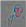
\includegraphics{pixmap/object_parts_2}}
    };
    \node(layer3rd3) [neuron,above=1.5 of layer2nd3] {
    	\scalebox{1.8}{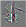
\includegraphics{pixmap/object_parts_3}}
    };
    
    \node(output1) [neuron,above=1.5 of layer3rd1] {
    	\Large 车
    };
    \node(output2) [neuron,above=1.5 of layer3rd2] {
    	\Large 人
    };
    \node(output3) [neuron,above=1.5 of layer3rd3] {
    	\Large 动物
    };
    
    \node [right=of input3] {
    	\large
    	\begin{tabular}{c}
	    	可见层\\
    		(输入像素)\\
    	\end{tabular}
    };

    \node [right=of layer1st3] {
    	\large
    	\begin{tabular}{c}
	    	第一个隐藏层\\
    		(边缘)\\
    	\end{tabular}
    };
    \node [right=of layer2nd3] {
    	\large
    	\begin{tabular}{c}
	    	第二个隐藏层\\
    		(角点和轮廓)\\
    	\end{tabular}
    };
    \node [right=of layer3rd3] {
    	\large
    	\begin{tabular}{c}
	    	第三个隐藏层\\
    		(物体组成部分)\\
    	\end{tabular}
    };
    \node [right=of output3] {
    	\large
    	\begin{tabular}{c}
	    	输出\\
    		(物体识别)\\
    	\end{tabular}
    };
	\node(image) [left=of layer2nd1,yshift=-1.6cm] {
		\scalebox{1.8}{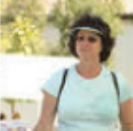
\includegraphics{pixmap/image_of_person}}
	};

	\foreach \x in {1,...,3}
		\foreach \y in {1,...,3} {
	  		\draw[thick,-{Latex[]}] (input\x) to (layer1st\y);
	  		\draw[thick,-{Latex[]}] (layer1st\x) to (layer2nd\y);
	  		\draw[thick,-{Latex[]}] (layer2nd\x) to (layer3rd\y);
	  		\draw[thick,-{Latex[]}] (layer3rd\x) to (output\y);
	};
	
	\draw[very thick,-{Latex[open]}] (image.south)++(1,0) .. controls(-3.5,-0.25) .. (input1.west);
	
  \end{tikzpicture}
\end{document}
